\documentclass[handout]{beamer}
\usepackage[utf8]{inputenc} 
\usepackage[T1]{fontenc}
\usepackage{lmodern}
\usepackage{graphicx}
\usepackage[french]{babel}
\usepackage{mathtools}
\usepackage{amsmath}
\usepackage{amssymb}
\usepackage{mathrsfs}
\usepackage{amsfonts}
\usepackage{geometry}
\usepackage{graphicx}

\usetheme{AnnArbor}
\everymath{\displaystyle}

\graphicspath{ {./images/} }

\title{Synthèse d’images 3D}
\subtitle{TIPE}
\author{Oscar Buon}

\setbeamertemplate{sidebar right}{}
\setbeamertemplate{footline}{
\hfill\usebeamertemplate***{navigation symbols}
\hspace{1cm}\insertframenumber{}/\inserttotalframenumber}

\begin{document}

\begin{frame}
    \maketitle
\end{frame}

\begin{frame}

    \frametitle{Objectifs}

    \begin{itemize}
        \item Concevoir un programme reposant sur l'algorithme du tracé de rayon afin de créer des images de synthèse.
        \item Optimiser le programme et augmenter la qualité des images.
        \item Utiliser la synthèse d'images 3D pour prévisualiser une pièce de bâtiment.
    \end{itemize}

\end{frame}

\begin{frame}
    \frametitle{Table des matières}
    \tableofcontents
\end{frame}

\section{Tracé de rayon}

\subsection{Problématique}

\begin{frame}
    Scène 3D : ensemble d'objets définis via des points, vecteurs et autres propriétés stockés dans la mémoire de l'ordinateur.

    Infographie 3D : créer une image matricielle 2D à partir d'une scène numérique 3D.

    Tracé de rayon : un algorithme permettant de faire de l'infographie 3D.
\end{frame}

\subsection{Modélisation}

\begin{frame}
    \begin{itemize}
        \item On modélise la lumière comme des rayons lumineux.
        \item Les objets sont délimités par des surfaces géométriques.
        \item Lorsqu'un rayon intersecte une surface, plusieurs choses peuvent se passer (absorption, réflexion, transmission...) en fonction des propriétés de l'objet.
    \end{itemize}
\end{frame}

\begin{frame}
    \frametitle{Modélisation de la lumière}
    \begin{figure}
        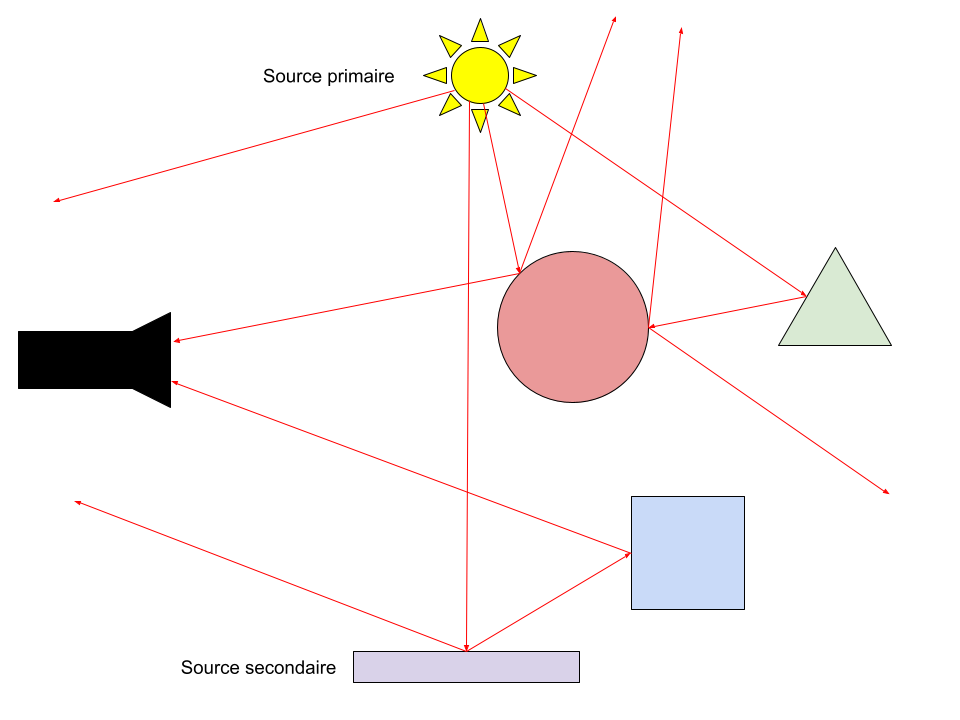
\includegraphics[scale=0.3]{Lumiere.png}
    \end{figure}
\end{frame}

\begin{frame}
    \frametitle{Principe de Fermat}
    \begin{figure}
        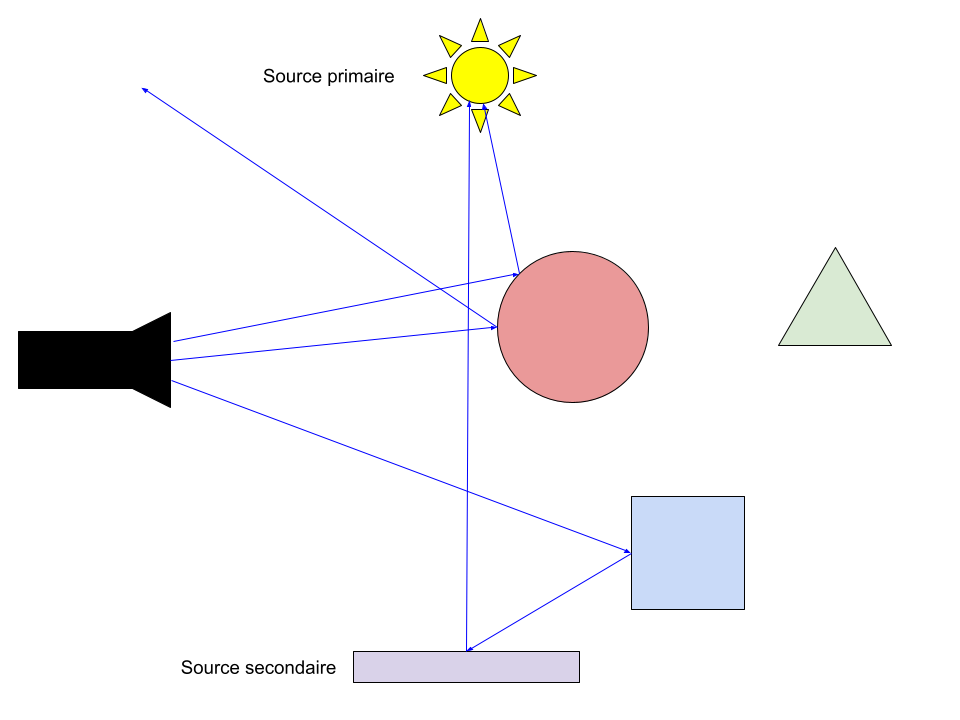
\includegraphics[scale=0.3]{Fermat.png}
    \end{figure}
\end{frame}

\subsection{Description de l'algorithme}

\begin{frame}
    \frametitle{Image matricielle}

    \begin{figure}
    \begin{tabular}{ | c | c | c | c | c | c | c | c | c | c | }
        \hline
        & & & & & & & & & \\
        \hline
        & & & & & & & & & \\
        \hline
        & & & & & & & & & \\
        \hline
        & & & & & & & & & \\
        \hline
        & & & & & & & & & \\
        \hline
        & & & & & & & & & \\
        \hline
        & & & & & & & & & \\
        \hline
        & & & & & & & & & \\
        \hline
        & & & & & & & & & \\
        \hline
        & & & & & & & & & \\
        \hline
    \end{tabular}
    \end{figure}

\end{frame}

\begin{frame}
    On définit une fonction de lancer de rayon qui à un point d'origine et une direction :
    \begin{itemize}
        \item Calcul quel est l'objet intersecté le plus proche.
        \item Récupère les propriétés optiques de l'objet.
        \item En fonction de celles-ci peut récursivement lancer de nouveaux rayons : rayon réfléchi, rayon transmis...
        \item Renvoie une information de couleur dépendant des propriétés de l'objet et des couleurs renvoyées par les nouveaux rayons.
    \end{itemize}
    Pour chaque pixel, on lance un rayon depuis la position de la caméra vers la direction du pixel.
    On obtient ainsi une image matricielle.
\end{frame}

\section{Implémentation et amélioration}

\begin{frame}

    \frametitle{Exemple}
    \begin{figure}
        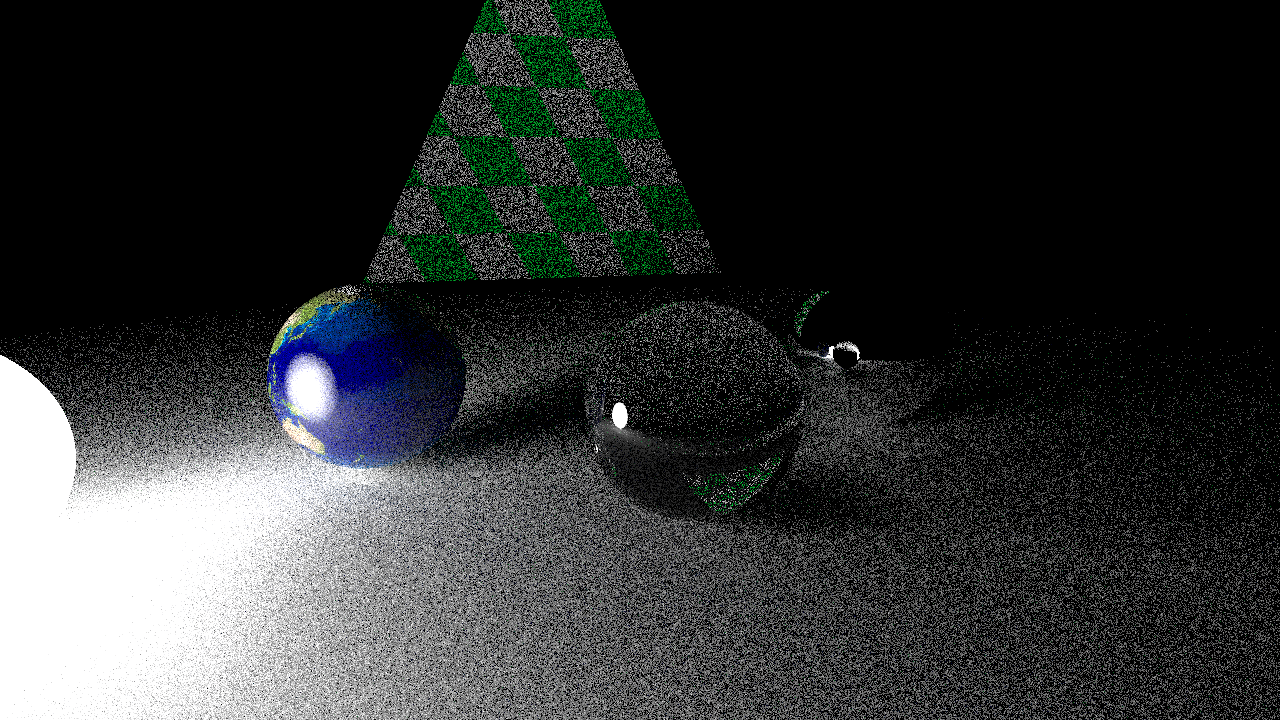
\includegraphics[scale=0.25]{night.png}
        \caption{100 samples, 105 seconds}
    \end{figure}
    
\end{frame}

\subsection{Parallélisation}

\begin{frame}

    En faisant tourner 4 instances de l'algorithme en parallèle fonctionnant sur 4 coeurs différents, on passe de 105 à 51 secondes.
    L'image reste la même.

\end{frame}

\subsection{Priorisation}

\begin{frame}

    \frametitle{Remarque}
    \begin{figure}
        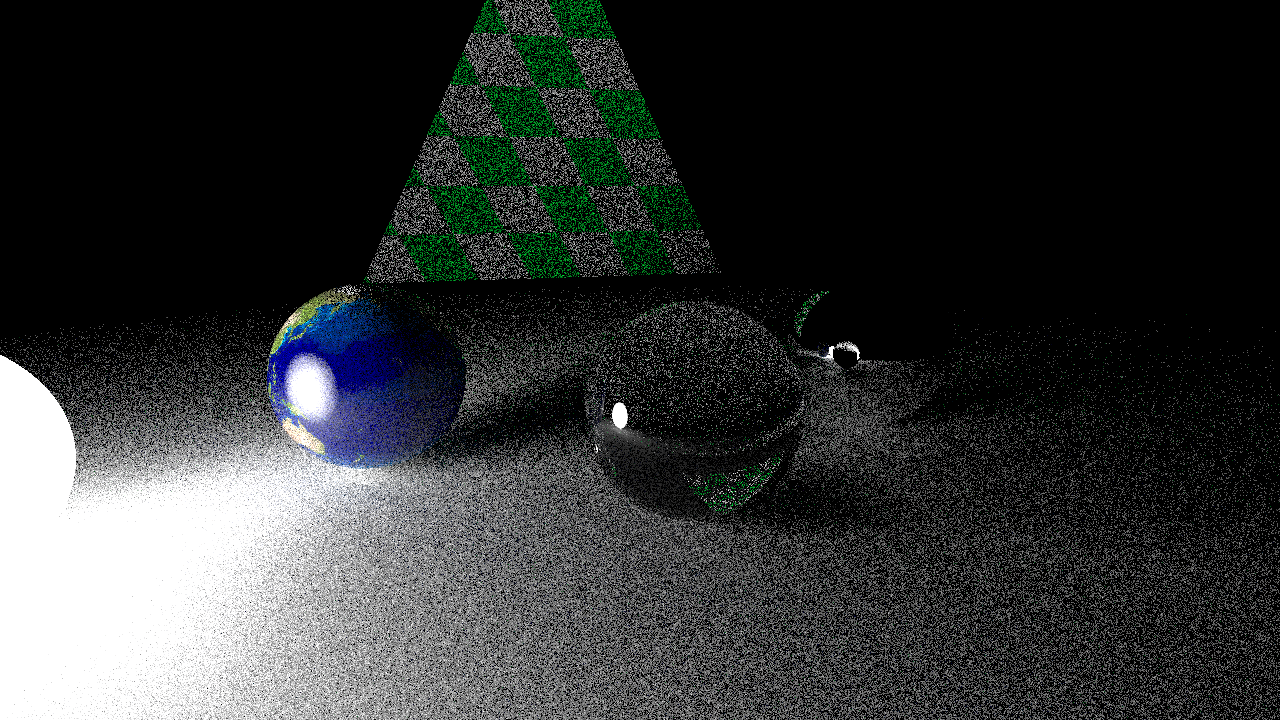
\includegraphics[scale=0.13]{night.png}
        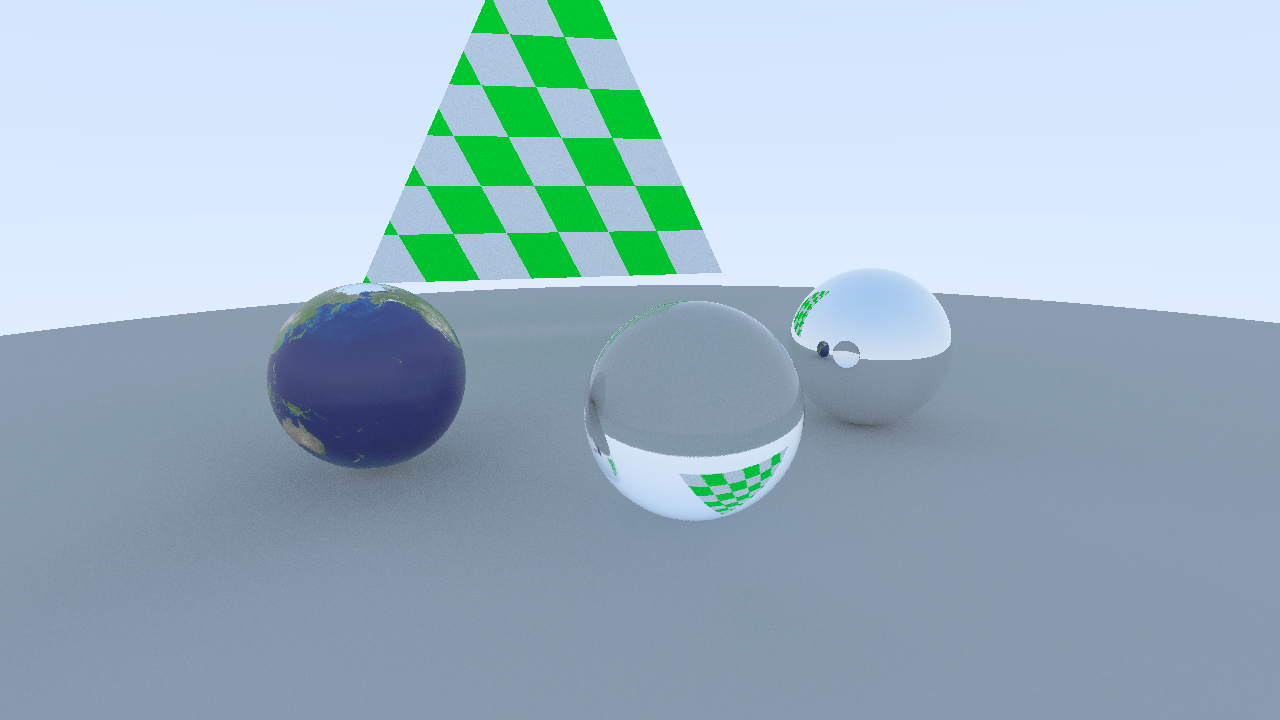
\includegraphics[scale=0.13]{day.png}
        \caption{100 samples, 50 seconds}
    \end{figure}

\end{frame}

\begin{frame}
    \frametitle{Objets diffus}
    \begin{figure}
        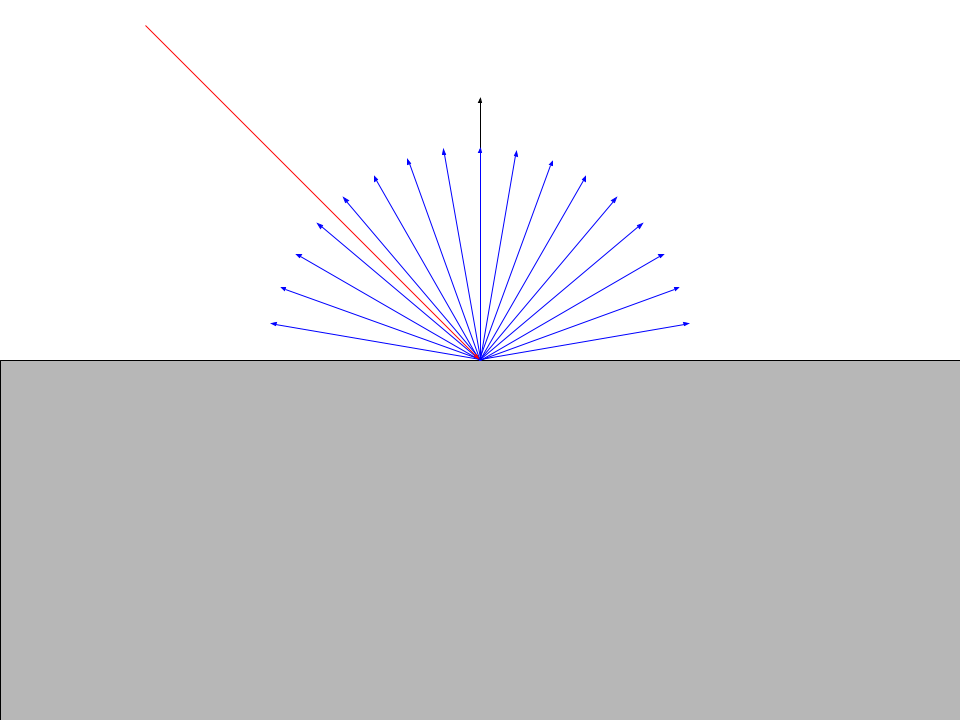
\includegraphics[scale=0.3]{Lambertian.png}
    \end{figure}
\end{frame}

\begin{frame}
    \frametitle{N'échantillonne pas la source lumineuse}
    \begin{figure}
        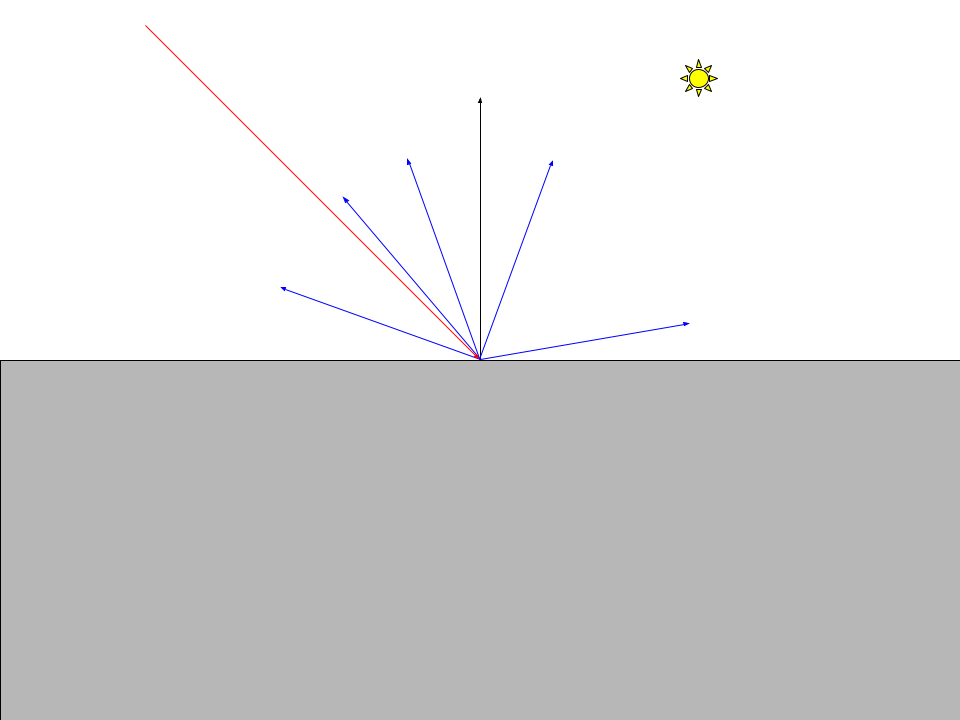
\includegraphics[scale=0.3]{Priority1.png}
    \end{figure}
\end{frame}

\begin{frame}
    \frametitle{Échantillonne la source lumineuse}
    \begin{figure}
        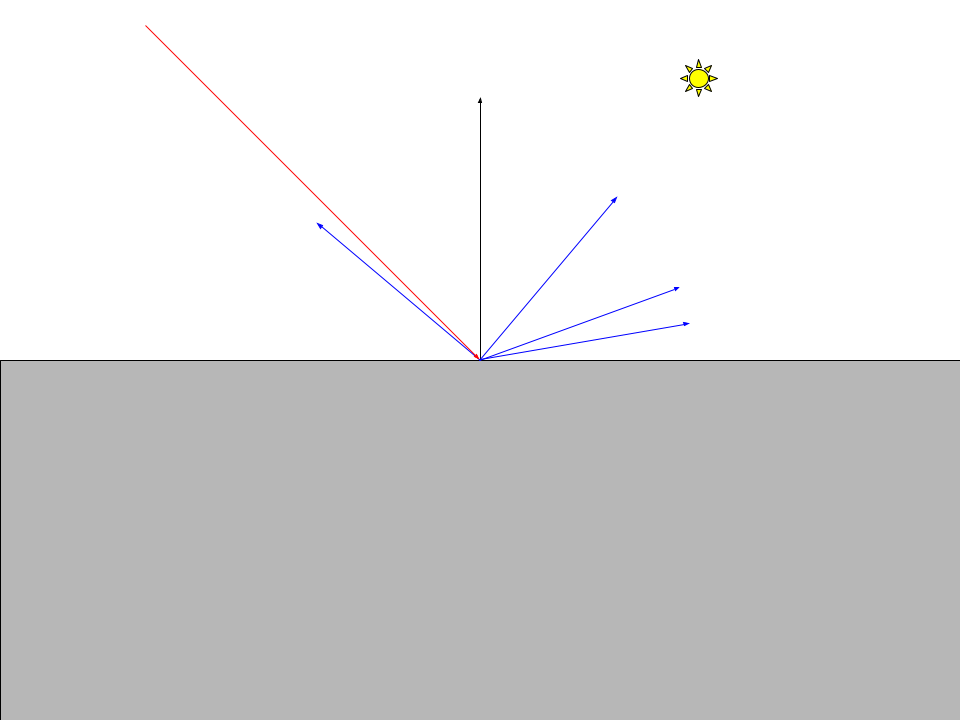
\includegraphics[scale=0.3]{Priority2.png}
    \end{figure}
\end{frame}

\begin{frame}
    \frametitle{Sans priorisation}

    \begin{figure}
        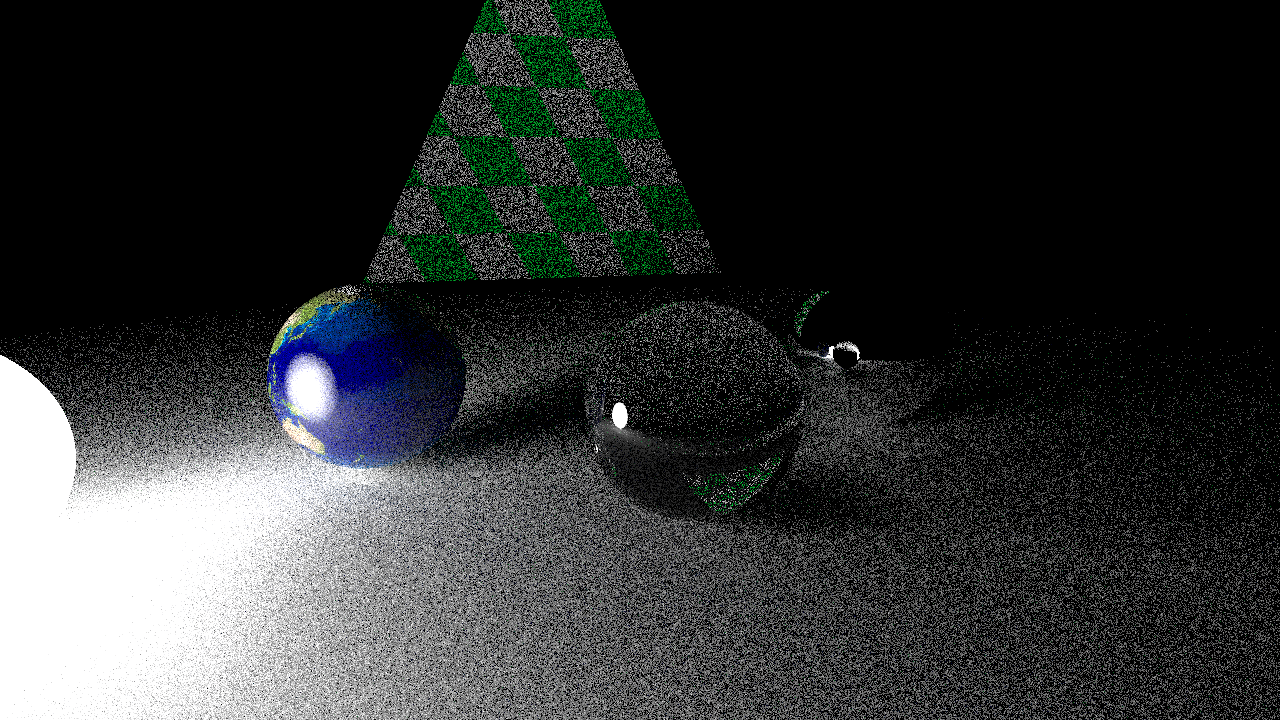
\includegraphics[scale=0.25]{night.png}
        \caption{100 samples, 50 seconds}
    \end{figure}

\end{frame}

\begin{frame}
    \frametitle{Avec priorisation}

    \begin{figure}
        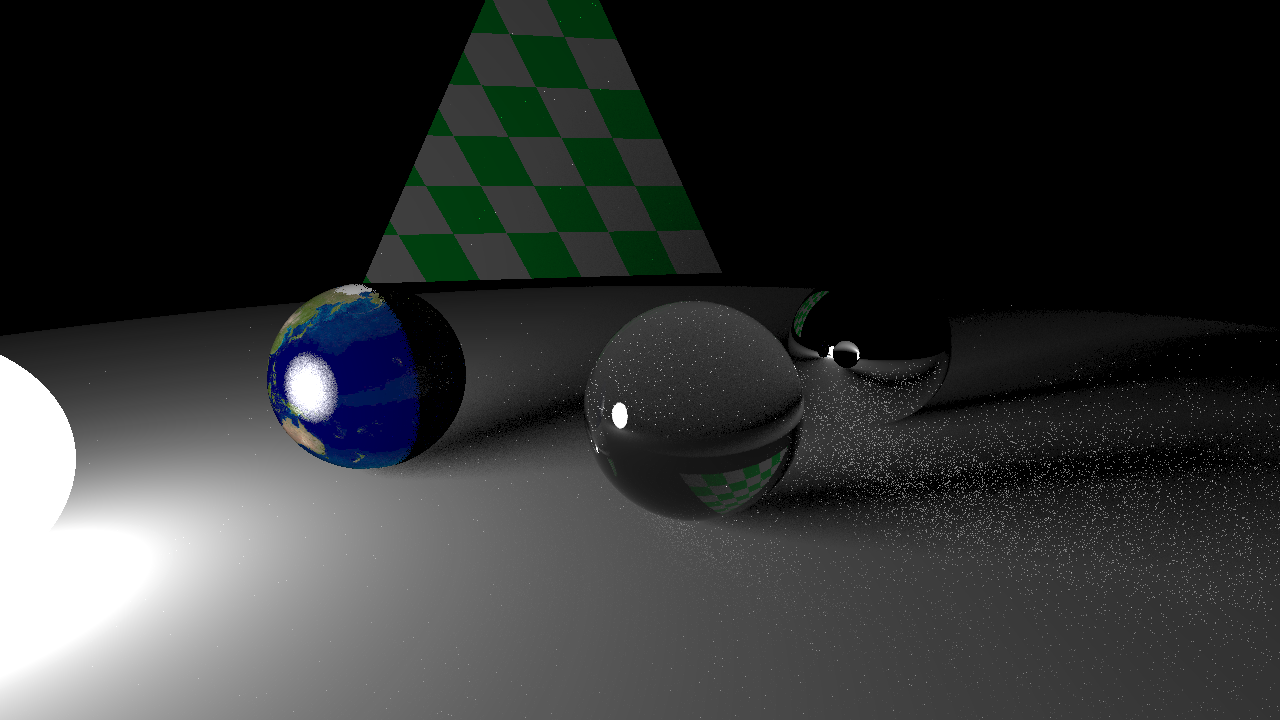
\includegraphics[scale=0.25]{priorisation.png}
        \caption{100 samples, priority 0.5, 46 seconds}
    \end{figure}

\end{frame}

\subsection{Traitement d'image}

\begin{frame}
    \frametitle{Idée}
    Produire une image plus rapidement mais de moins bonne qualité, pour ensuite l'améliorer avec des algorithmes de traitement d'images.
\end{frame}

\begin{frame}
    \frametitle{Sans traitement}

    \begin{figure}
        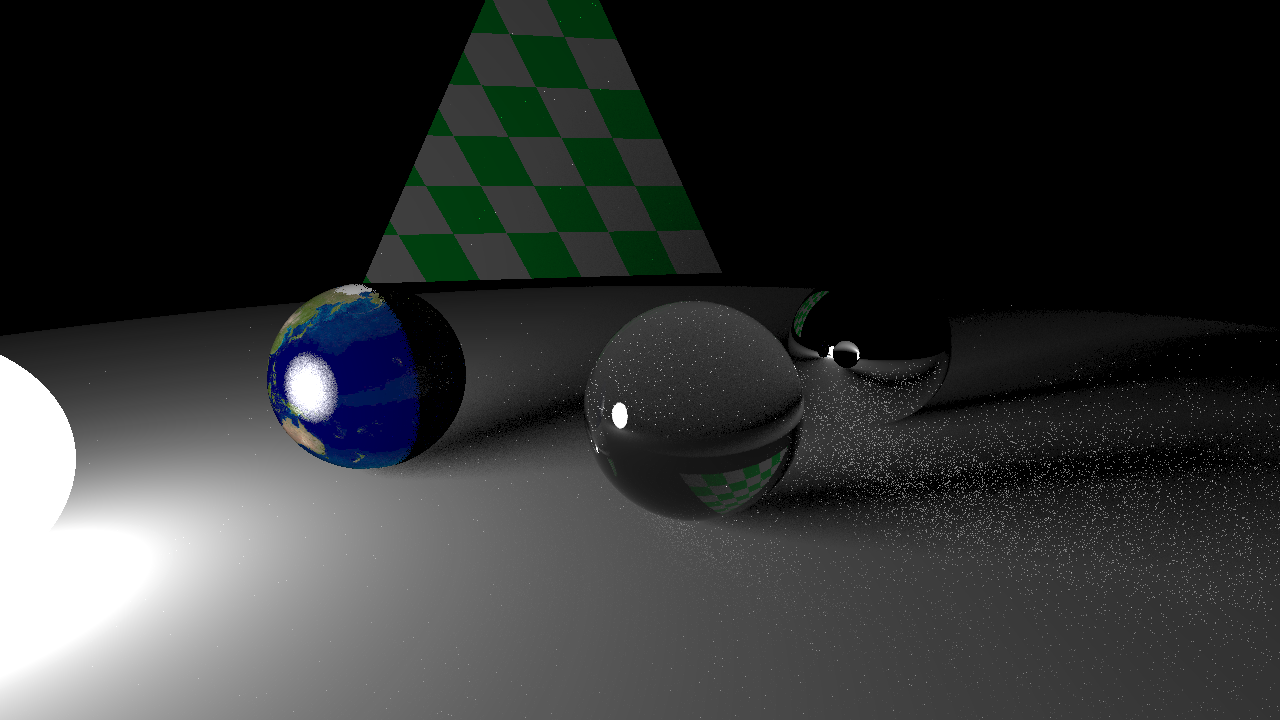
\includegraphics[scale=0.25]{priorisation.png}
        \caption{100 samples, priority 0.5, 46 seconds}
    \end{figure}

\end{frame}

\begin{frame}
    \frametitle{Avec filtre gaussien}

    \begin{figure}
        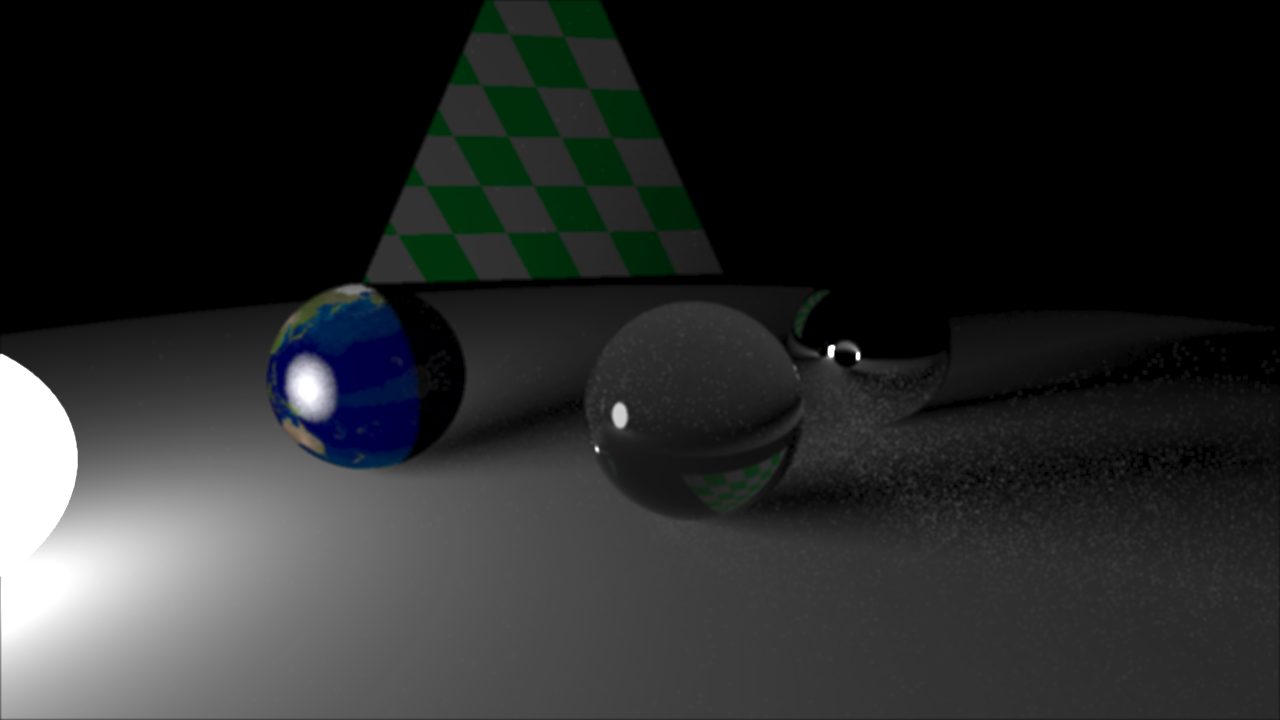
\includegraphics[scale=0.25]{gaussian5.png}
        \caption{100 samples, priority 0.5, gaussian 5/1.6, 49 seconds}
    \end{figure}

\end{frame}

\begin{frame}
    \frametitle{Avec filtre gaussien}

    \begin{figure}
        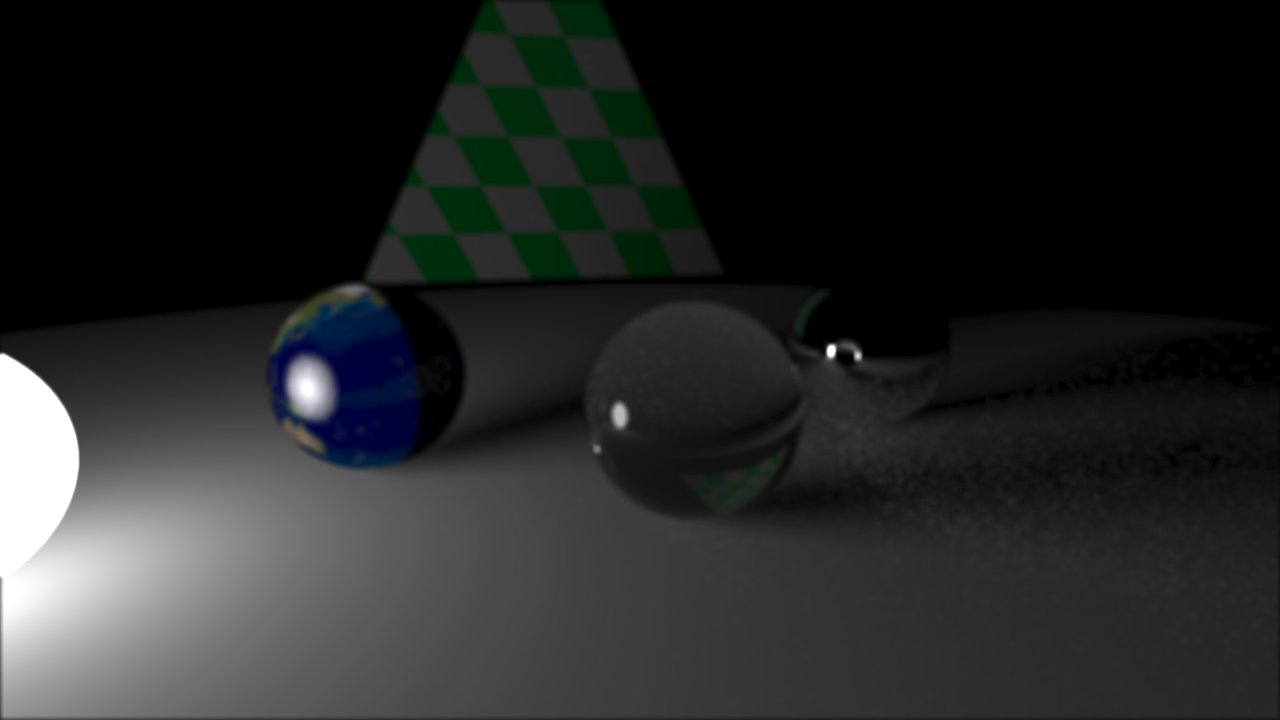
\includegraphics[scale=0.25]{gaussian10.png}
        \caption{100 samples, priority 0.5, gaussian 10/3.2, 56 seconds}
    \end{figure}

\end{frame}

\begin{frame}
    \frametitle{Un algorithme plus avancé}

    \begin{itemize}
        \item On sépare l'image en deux parties : la couleur propre des objets et leur illumination.
        \item On applique un filtrage à l'illumination seulement  :
        \begin{itemize}
            \item Filtre médian : pour chaque pixel, on prend la médiane des pixels voisins.
            \item Filtre gaussien : chaque pixel est moyenné avec ses voisins avec un coefficient
                $ G(x,y) = \frac{ e^{ \frac{x^2+y^2}{2 \sigma^2} } }{2 \pi \sigma^2} $.
        \end{itemize}
        \item On fusionne les deux images.
    \end{itemize}

\end{frame}

\begin{frame}
    \frametitle{Sans traitement}

    \begin{figure}
        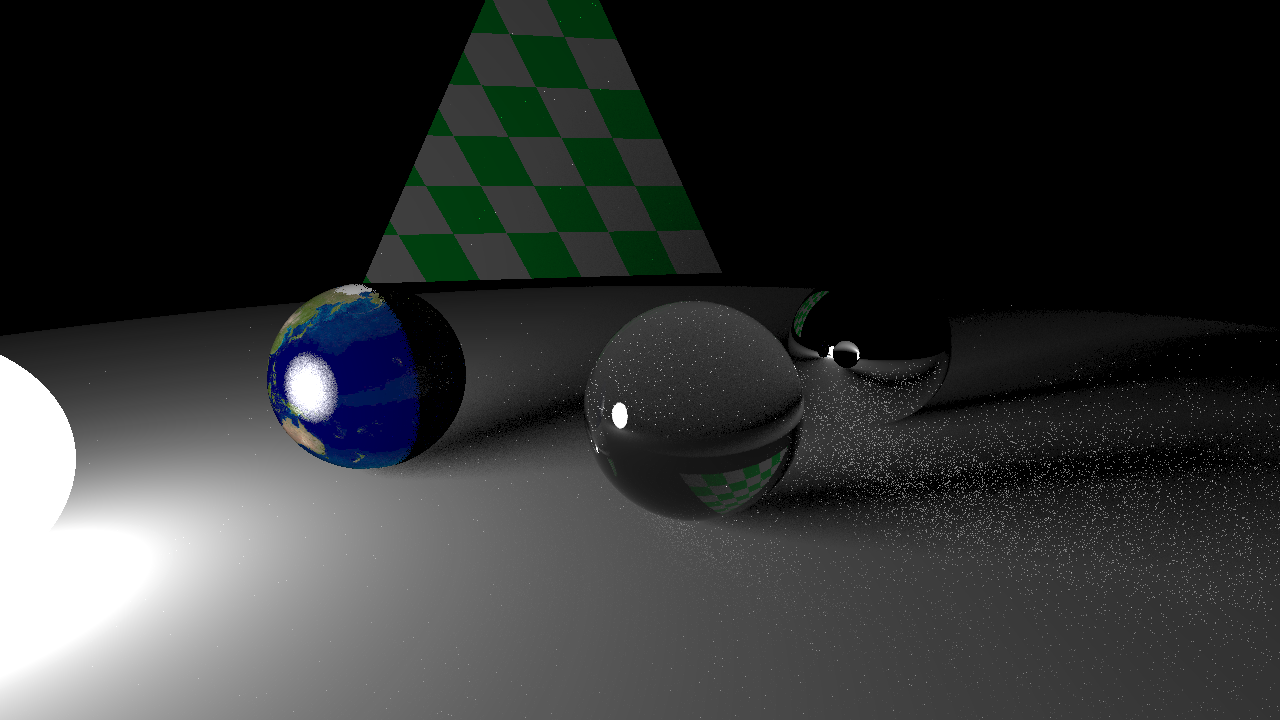
\includegraphics[scale=0.25]{priorisation.png}
        \caption{100 samples, priority 0.5, 46 seconds}
    \end{figure}

\end{frame}

\begin{frame}
    \frametitle{Avec traitement}

    \begin{figure}
        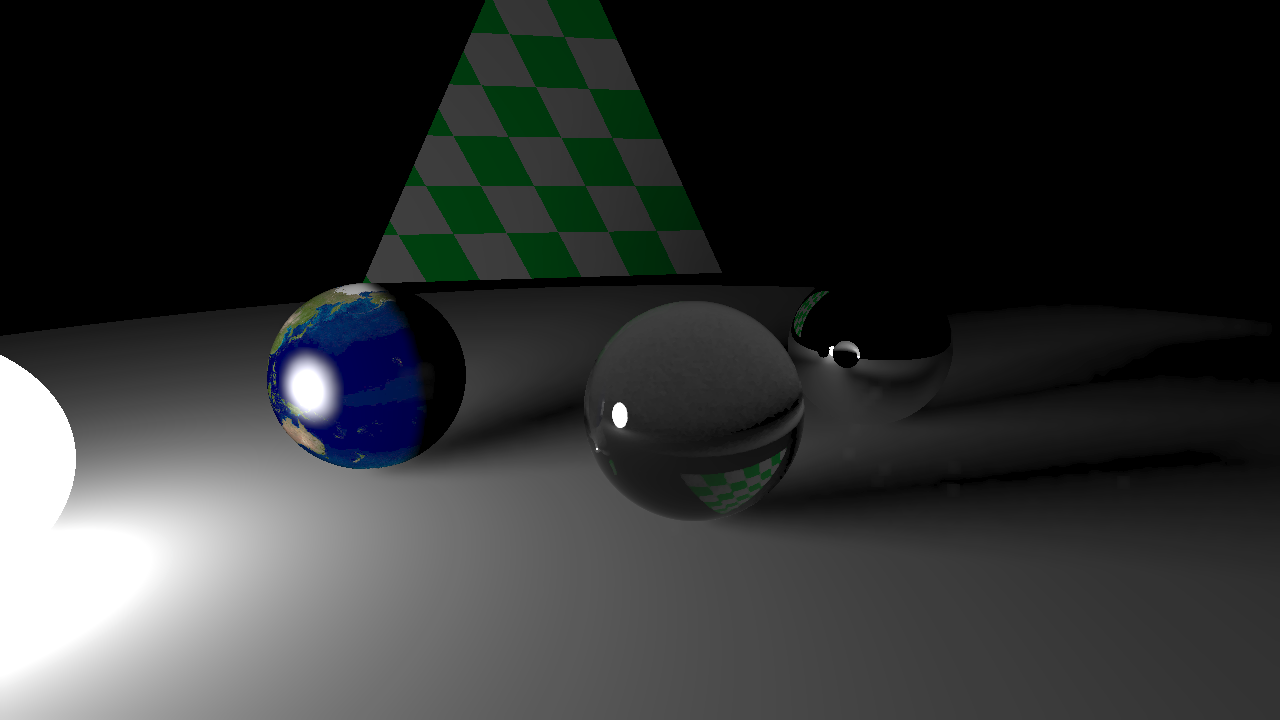
\includegraphics[scale=0.25]{processing.png}
        \caption{100 samples, priority 0.5, processing 2/0.8, 62 seconds}
    \end{figure}

\end{frame}

\subsection{Tests d'intersection}

\begin{frame}
    \frametitle{Idée}
    En rangeant intelligemment les objets, on pourrait limiter le nombre de tests d'intersection.
\end{frame}

\begin{frame}
    \frametitle{Bounding Volume Hierarchy (BVH)}
    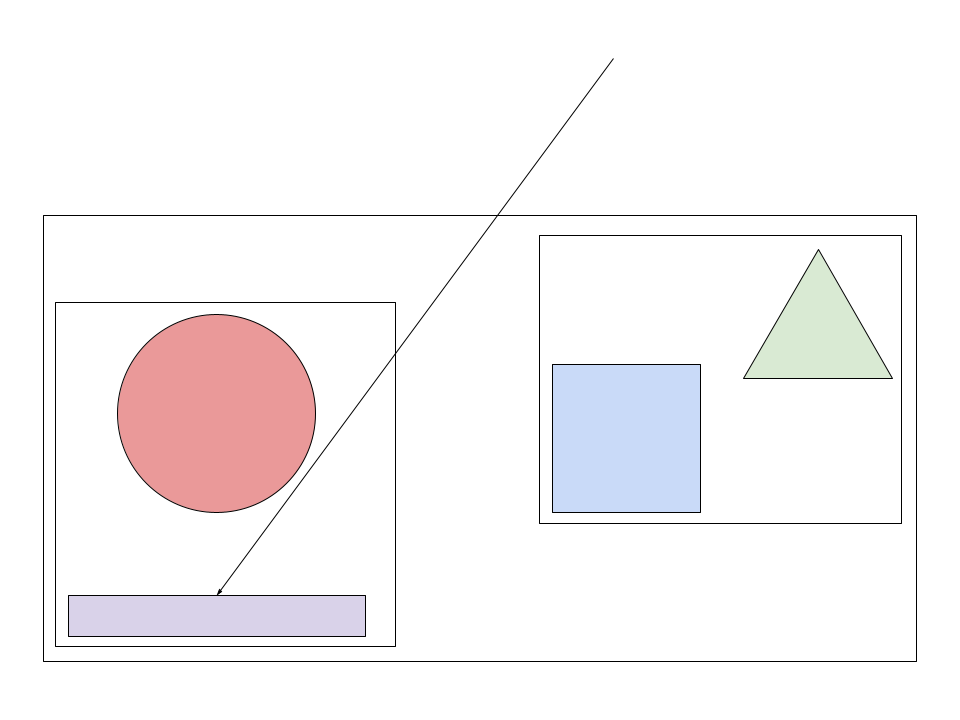
\includegraphics[scale=0.3]{Arbre.png}
\end{frame}

\begin{frame}
    \frametitle{Comparaison}

    \begin{figure}
        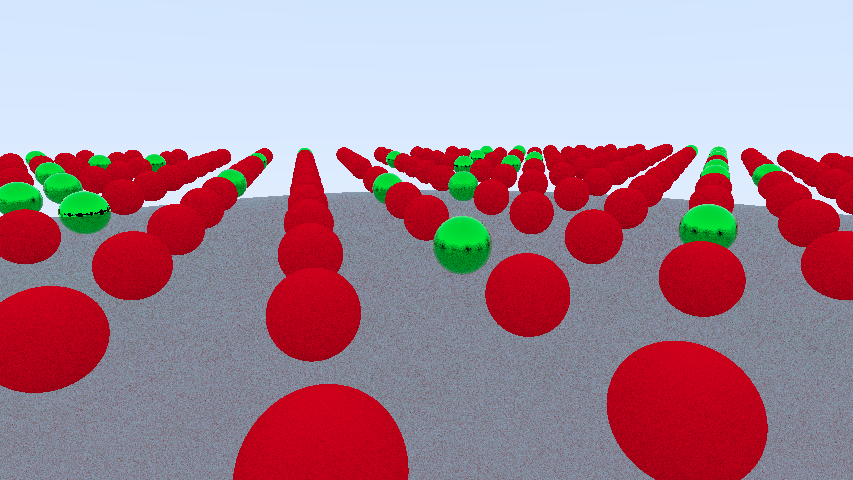
\includegraphics[scale=0.2]{bvh.png}
        \caption{Pour une scène avec 400 sphères et 10 échantillons par pixel, on passe de 96 à 58 secondes.}
    \end{figure}

\end{frame}

\section{Résultat final}

\subsection{Application}

\begin{frame}
    \frametitle{Pièce de bâtiment avec murs en bricks}

    \begin{figure}
        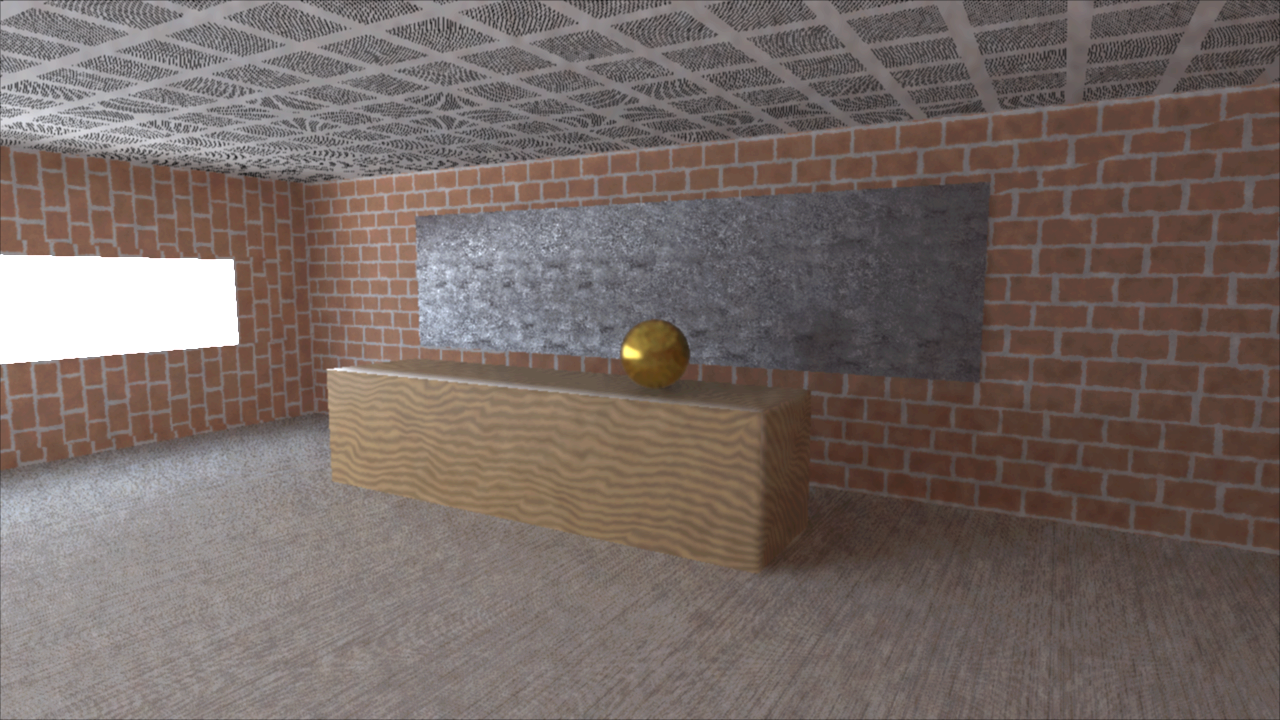
\includegraphics[scale=0.25]{piece_bricks.png}
        \caption{100 samples, processing 2/0.8, 1274 seconds, average 0.148}
    \end{figure}

\end{frame}

\begin{frame}
    \frametitle{Pièce de bâtiment avec murs peints}

    \begin{figure}
        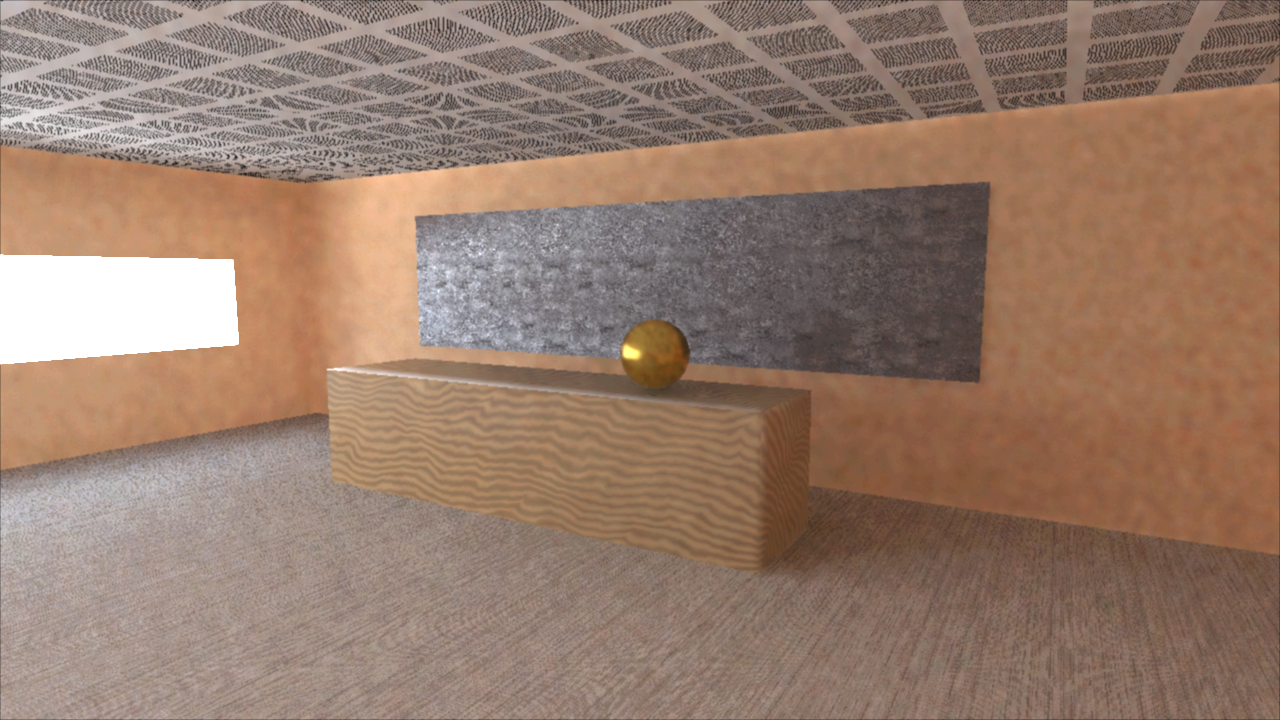
\includegraphics[scale=0.25]{piece_peinture.png}
        \caption{100 samples, processing 2/0.8, 1224 seconds, average 0.172}
    \end{figure}

\end{frame}


\begin{frame}
    \frametitle{Tableau moins rugueux}

    \begin{figure}
        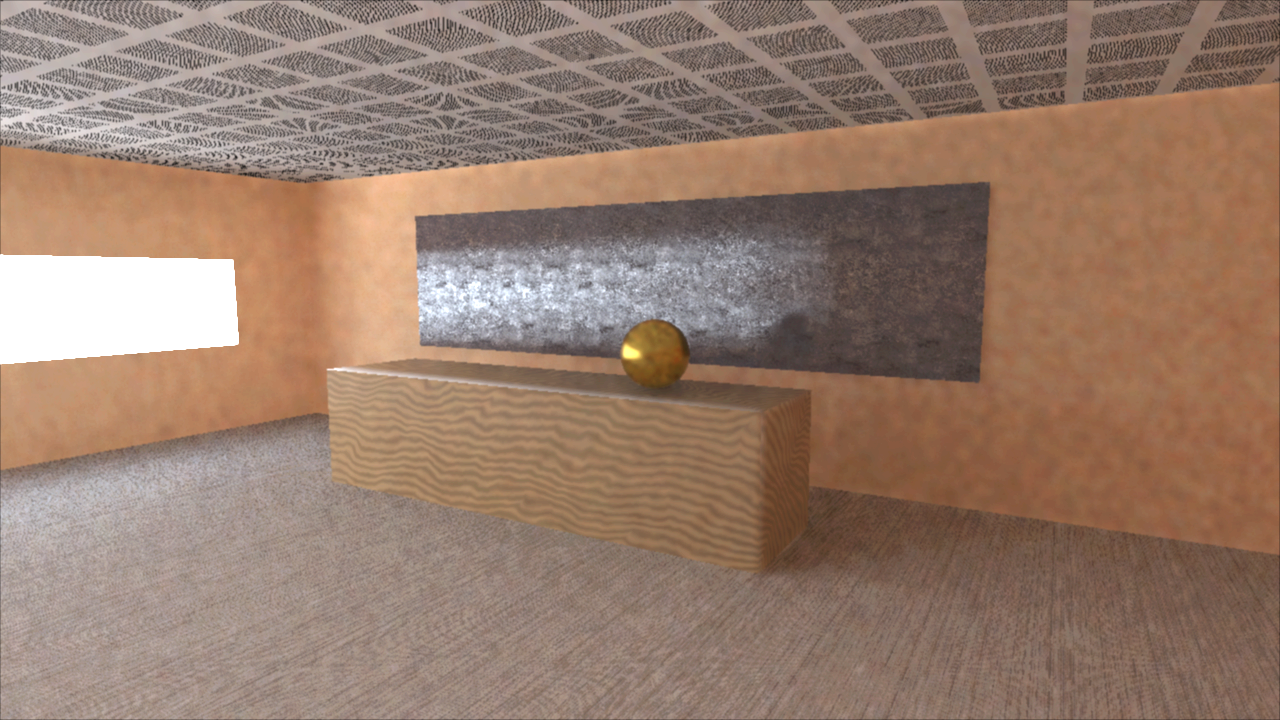
\includegraphics[scale=0.25]{tableau.png}
        \caption{100 samples, processing 2/0.8, 1418 seconds, average 0.172}
    \end{figure}

\end{frame}

\subsection{Conclusion}

\begin{frame}
    \frametitle{Conclusion et pistes d'améliorations}

    \begin{itemize}
        \item L'implémentation de l'algorithme fonctionne.
        \item Il est possible de l'utiliser dans le domaine de l'architecture.
        \item
            Le programme a pu être optimisé, cependant pas suffisamment pour être utilisé en temps réel.
            Il existe tout de même plusieurs pistes d'améliorations :
            \begin{itemize}
                \item utiliser l'accélération matérielle ;
                \item précalculer certains éléments.
            \end{itemize}
    \end{itemize}

\end{frame}

\subsection{Annexe}

\begin{frame}
    \frametitle{Pièce de bâtiment avec murs peints}

    \begin{figure}
        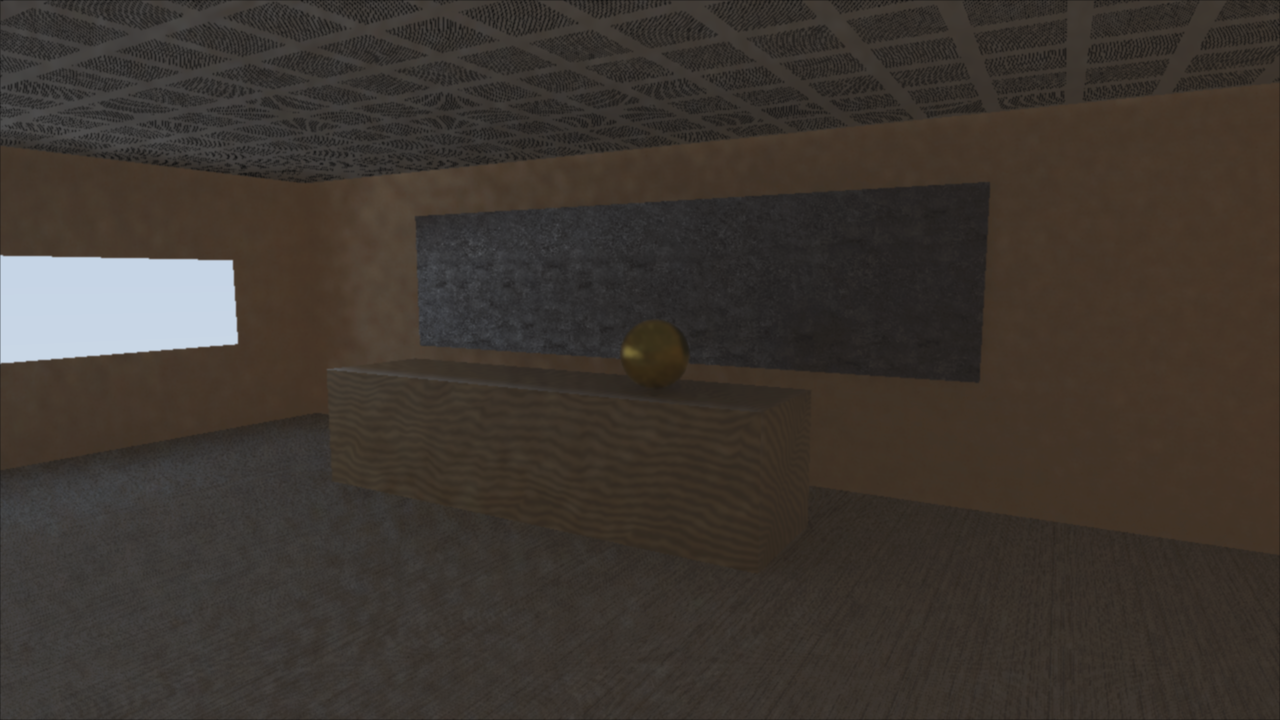
\includegraphics[scale=0.25]{piece_peinture_triche.png}
        \caption{light 0.172, 25 samples, processing 2/0.8, 70 seconds, average 0.201}
    \end{figure}

\end{frame}


\begin{frame}

    \frametitle{Physicaly Based Rendering (PBR)}

    Comment modéliser la lumière de manière physiquement plausible ?

    Les critères du PBR :
    \begin{enumerate}
        \item Définir pour chaque surface une valeur de rugosité.
        \item Respecter le principe de conservation de l'énergie lumineuse.
        \item Se baser sur une fonction de réflectivité bidirectionnelle.
    \end{enumerate}
    
\end{frame}

\begin{frame}

    \frametitle{Grandeurs importantes}

    L'énergie $ Q = \frac{hc}{\nu} $ en $ J $.

    La puissance ou flux $ \Phi = \frac{\partial Q}{\partial t} $ en $ W $.

    L'irradiance et l'exitance $ E = \lim_{\Delta A \to 0}  \frac{\Delta \Phi }{\Delta A} $ en $W.m^{-2} $.

    La luminance $ L = \lim_{\Delta \omega \to 0}  \frac{\Delta E }{\Delta \omega } $ en $ W.m^{-2}.sr^{-1} $.
\end{frame}

\begin{frame}

    \frametitle{Équation de rendu}

    \begin{align*}
        L_o(x, \omega_o, \lambda, t)
        &= L_e(x, \omega_o, \lambda, t) \\
        &+ \int_{\Omega}^{} f(x, \omega_i, \omega_0, \lambda, t)
        L_i(x, \omega_i, \lambda, t)
        (\omega_i . n) d\omega_i
    \end{align*}

\end{frame}

\begin{frame}
    \frametitle{Lambertien}
    \begin{figure}
        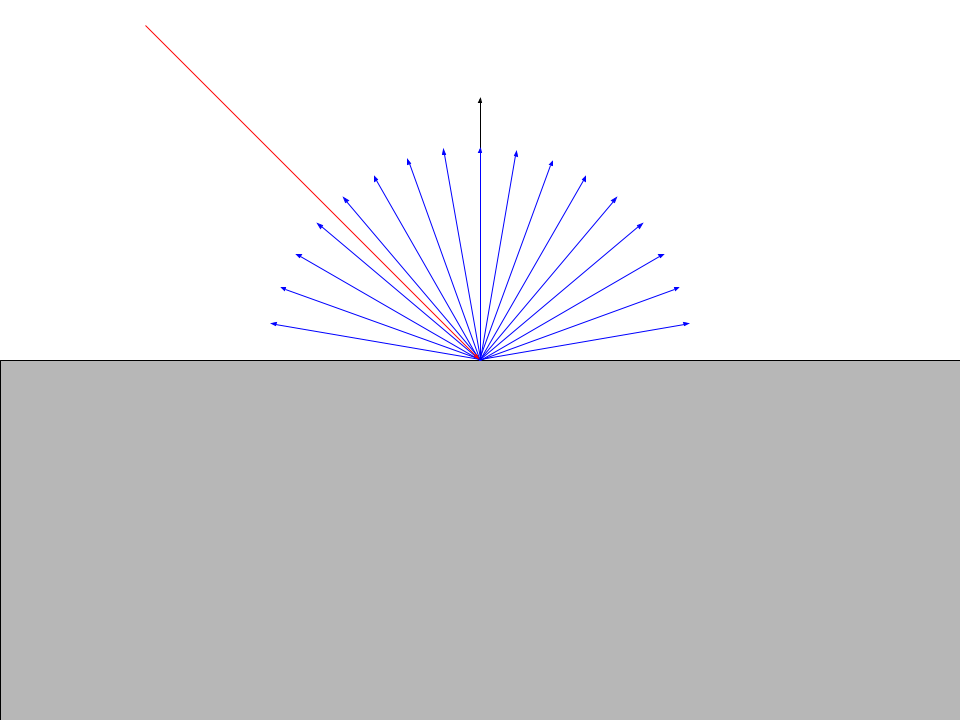
\includegraphics[scale=0.3]{Lambertian.png}
    \end{figure}
\end{frame}

\begin{frame}
    \frametitle{Réflexion spéculaire}
    \begin{figure}
        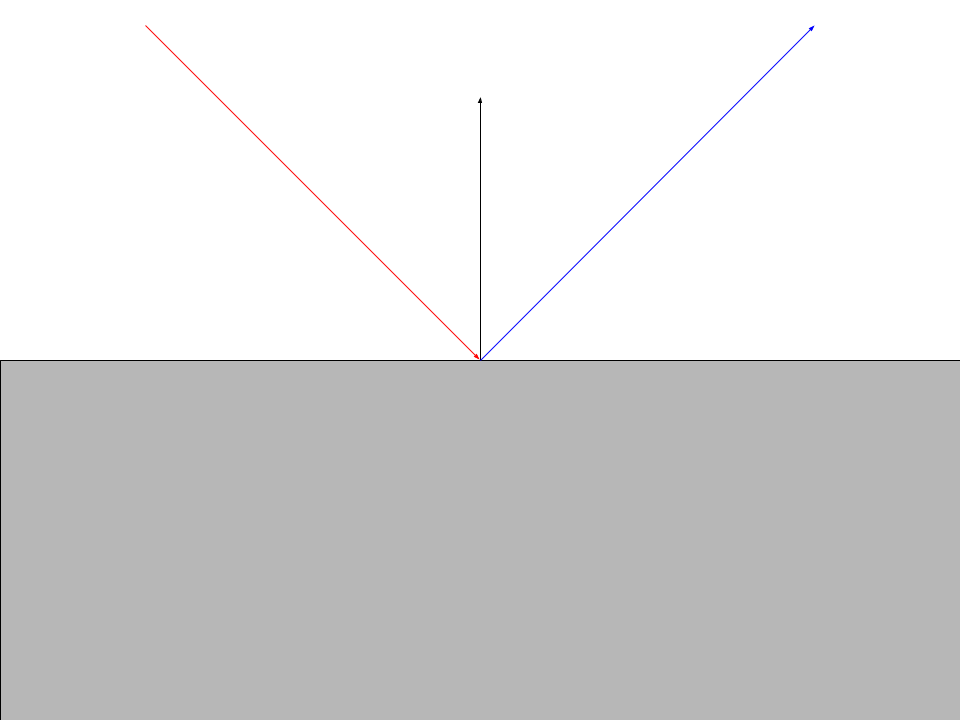
\includegraphics[scale=0.3]{Metal.png}
    \end{figure}
\end{frame}

\begin{frame}
    \frametitle{Transmission spéculaire}
    \begin{figure}
        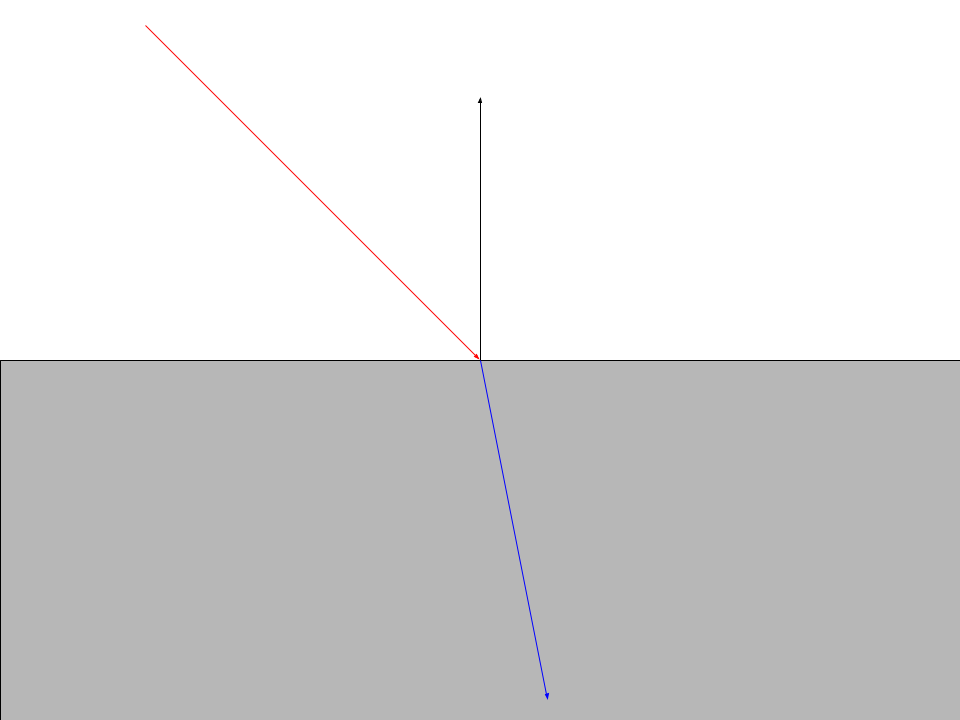
\includegraphics[scale=0.3]{Dielectrique.png}
    \end{figure}
\end{frame}

\begin{frame}
    \frametitle{Lampe}
    \begin{figure}
        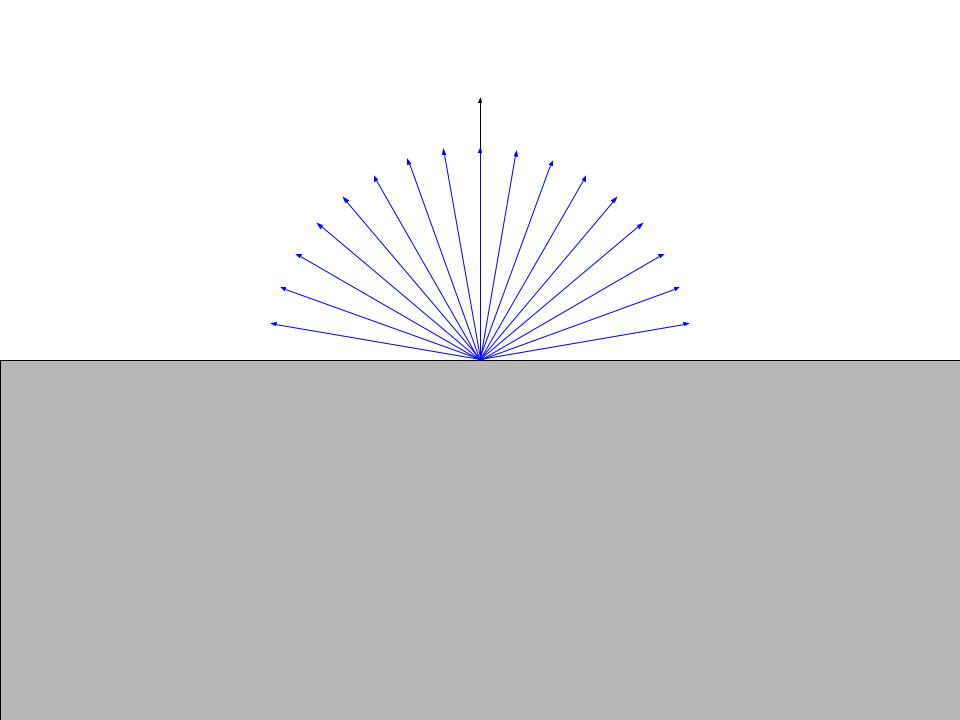
\includegraphics[scale=0.3]{Lampe.png}
    \end{figure}
\end{frame}

\begin{frame}
    On peut modéliser une surface réflexive réelle avec un nombre restreint de paramètres :
    \begin{itemize}
        \item Spectre diffus
        \item Spectre spéculaire
        \item Spectre émis
        \item Rugosité
        \item Normale
    \end{itemize}
\end{frame}

\end{document}